%===============================================================================
% DOCUMENT
%===============================================================================

%% Document class
\documentclass[a4paper,12pt]{scrreprt}

%% Include packages
\usepackage{packages}

\begin{document}

%% Include custom commands
\include{commands}

\pagenumbering{gobble}

%% Build cover
\definecolor{titlepagecolor}{RGB}{37,64,56}

%==========================================================================
% COLORED BAR ON THE LEFT SIDE
%==========================================================================

\backgroundsetup{
    scale=1,
    angle=0,
    opacity=1,
    contents={
        \begin{tikzpicture}[remember picture,overlay]
            \path [fill=titlepagecolor] (-10.5,-15) rectangle ++ (5,30);
            \node[color=white] at (-6.90,-11.5) {\bfseries {\fontsize{120}{60} \textsf{C}}};
            \node[color=titlepagecolor] at (-4.30,-11.5) {\bfseries {\fontsize{120}{60} \textsf{C}}};
        \end{tikzpicture}
    }
}

%==========================================================================
% COVER PAGE CONTENT
%==========================================================================

\title{\LARGE{Network Monitoring System}}

\author{
    Flávia Alexandra da Silva Araújo (A96587)\\ \quad
    Joshua David Amaral Moreira (A105684)\\ \quad
    Miguel Torres Carvalho (A95485)\\ \quad
}

%% Date
\date{\today}

%% Course
\newcommand{\Course}{Licenciatura em Engenharia Informática}

%% Department
\newcommand{\Department}{Escola de Engenharia}

%% UniName
\newcommand{\UniName}{Universidade do Minho}

%% UniPic
\newcommand{\UniPic}{
\includegraphics[width=120pt]{img/eeum.png}}

%% University
\newcommand{\University}{
    \begin{flushleft}
        \UniPic
    \end{flushleft}
    \textcolor{gray}{\small\textbf{\textsf{\UniName}}}\par
    \textcolor{gray!80!white}{\small{\textsf{\Department}}}\par
    \textcolor{gray!70!white}{\small{\textsf{\Course}}}
}

%% UC
\newcommand{\UC}{
    \begin{flushleft}
        \par\textcolor{titlepagecolor}{\Large\textbf{\textsf{Comunicações por Computador}}}
    \end{flushleft}
}

%% Project Phase
\newcommand{\SubTitle}{
    \begin{flushleft}
        \large\textbf{Trabalho Prático 2}
    \end{flushleft}
}

%% Group Info
\newcommand{\GroupInfo}{\par Grupo 10 - PL1}

%% GitHub Repo
\newcommand{\GitHubRepo}{\par\url{https://github.com/migueltc13/CC-tp2}}

%% School Year
\newcommand{\SchoolYear}{
    \par\small{\textsf{Ano Letivo de 2024/2025}}
}

%% Define new command to show title, author and date
\makeatletter
\let\Title\@title
\let\Author\@author
\let\Date\@date
\makeatother

%==========================================================================
% BEGIN COVER PAGE
%==========================================================================

%% Make cover page
\newcommand{\makecover}{

%% Removes page number on footer
\thispagestyle{empty}

%% No indentation
\setlength{\parindent}{0em}

%% Put Background defined on \backgroundsetup, in this page
\BgThispage

%% Changing geometry to prevent overlay with text
%% At the end of back cover, geometry is default with \restoregeometry
\newgeometry{top=4cm,left=6cm,right=2cm,bottom=2cm}

%% builds university info defined previously
\University
\vspace{1cm}
\UC
\SubTitle
\SchoolYear

\vspace*{4cm}
%% bigger space (i think its the default one) between paragraphs
\setlength{\parskip}{1em}

%% builds title info defined previously
\par\textbf{\textsf{\huge\Title}}
\vspace{1cm}
%% builds author(s) info defined previously
\par\Author

\vspace{0.5cm}

%% builds date info defined previously
\par\Date
\restoregeometry
\pagebreak

}

%==========================================================================
% END COVER PAGE
%==========================================================================

\makecover

%% Default geometry
\newgeometry{top=3cm,left=3cm,right=3cm,bottom=4cm}

%% Save default geometry
\savegeometry{default}

%% Load default geometry with:
% \loadgeometry{default}

%===============================================================================
% BEGIN ABSTRACT PAGE
%===============================================================================

\renewenvironment{abstract}
 {\par\noindent\textbf{\Large\abstractname}\par\bigskip}
 {}

\begin{flushleft}
\begin{abstract}
    \par No presente relatório, é apresentada a solução desenvolvida para a Unidade Curricular
    de \textbf{Comunicações por Computador}, como parte do projeto final do semestre -
    \textbf{\textit{Network Monitoring System}}.
    Este trabalho teve como objetivo projetar um sistema capaz de monitorizar
    o tráfego de rede, bem como o desempenho dos dispositivos, entre um servidor
    centralizado e vários agentes distribuídos, permitindo a execução de tarefas
    de monitorização, com a respetiva recolha de métricas de desempenho e envio
    de alertas previamente configurados.

    No sistema desenvolvido implementaram-se dois protocolos aplicacionais: \\
    \textbf{\textit{AlertFlow}}:
    destinado ao envio de alertas quando certas condições de monitorização
    definidas são excedidas, utilizando, como protocolo de transporte,
    o \textit{Transmission Control Protocol} (TCP). \\
    \textbf{\textit{NetTask}}: implementado para a comunicação de tarefas de monitorização
    e recolha de métricas, sobre o \textit{User Datagram Protocol} (UDP),
    este protocolo aplicacional foi desenvolvido de forma a assegurar
    a comunicação robusta e confiável entre o servidor e os agentes.

    O trabalho foi concluído com a implementação e validação das principais funcionalidades do sistema,
    demonstrando a sua eficácia em ambientes de teste representativos em ambientes virtualizados.
    Este relatório documenta detalhadamente o \textit{design}, implementação, utilização
    e resultados obtidos.

\par \textbf{Palavras-Chave}: \textit{Network Monitoring System}, TCP, UDP,
    \textit{AlertFlow}, \textit{NetTask}, \textit{python3}, \textit{iperf3},
    \textit{ping}, \textit{Comunicações por Computador}.
\end{abstract}
\end{flushleft}

\pagebreak

%===============================================================================
% END ABSTRACT PAGE
%===============================================================================

%===============================================================================
% BEGIN INDEXES PAGES
%===============================================================================

%% Changes table of content name
\renewcommand{\contentsname}{Índice}
\renewcommand{\listfigurename}{Índice de Figuras}
\renewcommand{\lstlistlistingname}{Índice de \textit{Snippets}}

\tableofcontents
\pagebreak

\listoffigures
\pagebreak

\lstlistoflistings
\pagebreak

%===============================================================================
% END INDEXES PAGES
%===============================================================================

\pagenumbering{arabic}

%===============================================================================
% BEGIN ARQUITETURA DA SOLUÇÃO
%===============================================================================

\chapter{Arquitetura da Solução}

\begin{minipage}{\textwidth}
    \centering
    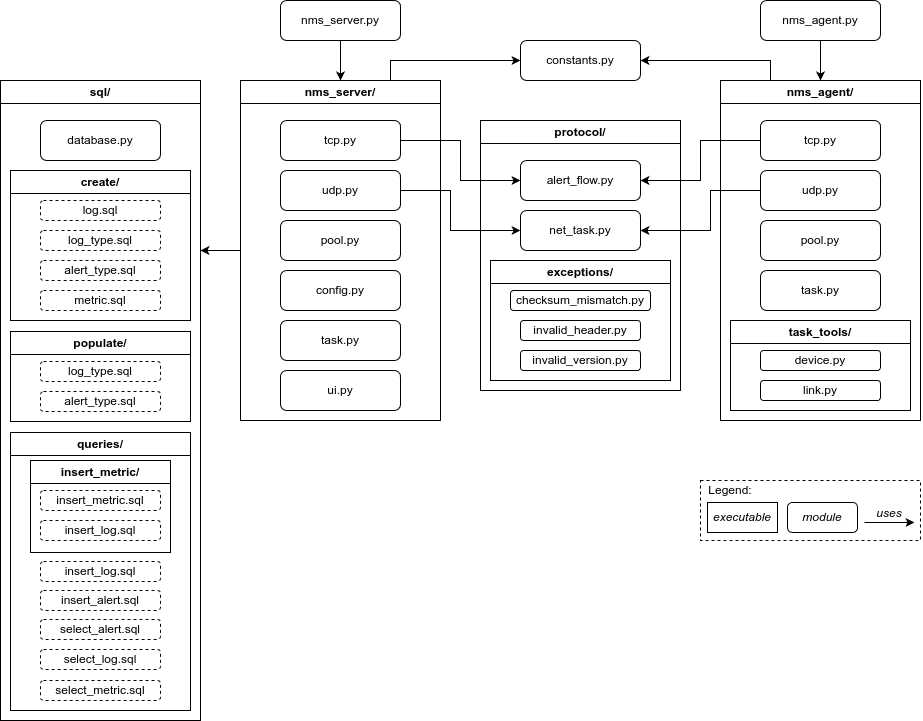
\includegraphics[width=\textwidth]{img/architecture.png}
    \captionof{figure}{Arquitetura da solução \textit{Network Monitoring System}}
    \label{fig:architecture}
\end{minipage}

%===============================================================================
% END ARQUITETURA DA SOLUÇÃO
%===============================================================================

%===============================================================================
% BEGIN ESPECIFICACÕES DOS PROTOCOLOS APLICACIONAIS
%===============================================================================

\newgeometry{top=0cm}

\chapter{Especificações dos Protocolos Aplicacionais}

\section{\textit{AlertFlow}}

\subsection{Formato de Mensagem}

\subsection{Diagrama de Sequência}

\begin{itemize}
    \item Normal
\end{itemize}

\loadgeometry{default}
\clearpage

\section{\textit{NetTask}}

O protocolo \textit{NetTask} é essencial para a funcionalidade harmonizada do
\textbf{\textit{Network Monitoring System}}, sendo este usado para a maioria
das comunicações entre o servidor e os agentes, tais como, a primeira conexão de
um agente ao servidor, o envio de tarefas pelo servidor, o envio de resultados
de tarefas pelos agentes, e a terminação de conexões nos dois sentidos.

Deste modo, o protocolo \textit{NetTask} foi desenvolvido para ser robusto e
adaptável a condições adversas de rede, garantindo a entrega fiável e integral
de mensagens, sobretudo em rotas deterioradas, com perdas ou duplicação de pacotes,
latências elevadas e taxas de débito variáveis.

Para combater tais adversidades, o protocolo aplicacional \textit{NetTask}
responsabiliza-se pelas funcionalidades que serão exploradas no seguinte
subcapítulo \nameref{subsec:nt_desc_funcionalidades}.

Nos próximos subcapítulos, serão detalhadas as especificações do protocolo,
nomeadamente o formato do cabeçalho e descrição dos respetivos campos,
descrição de funcionalidades e diagramas de sequência que ilustram o
comportamento do protocolo em situações normais e adversas.

\subsection{Formato de Cabeçalho e Descrição de Campos}

\begin{minipage}{\textwidth}
    \centering
    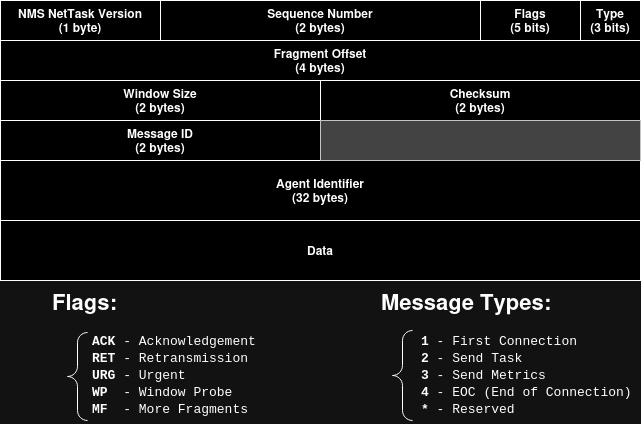
\includegraphics[width=\textwidth]{img/nettask_header.png}
    \captionof{figure}{Formato do cabeçalho do protocolo \textit{NetTask}}
    \label{fig:nettask_message_format}
\end{minipage}

\begin{itemize}
    \item \textbf{\textit{NMS NetTask Version}} (1 \textit{byte}):  versão do protocolo,
        para assegurar a compatibilidade de versões entre o servidor e os agentes;
    \item \textbf{\textit{Sequence Number}}     (2 \textit{bytes}): número de sequência da mensagem,
        para a ordenação de pacotes, deteção de pacotes duplicados e identificação de \textit{acknowledgements};
    \item \textbf{\textit{Flags}}               (5 \textit{bits}):  \textit{flags} de controlo:
        \begin{itemize}
           \item [\textbf{\textit{ACK}}] (1º \textit{bit}): \textit{Acknowledgement}, utilizado para confirmar a receção de pacotes;
           \item [\textbf{\textit{RET}}] (2º \textit{bit}): \textit{Retransmission}, indica que o pacote é uma retransmissão;
           \item [\textbf{\textit{URG}}] (3º \textit{bit}): \textit{Urgent}, indica que a mensagem é urgente;
           \item [\textbf{\textit{WP}} ] (4º \textit{bit}): \textit{Window Probe}, utilizado para o controlo de fluxo;
           \item [\textbf{\textit{MF}} ] (5º \textit{bit}): \textit{More Fragments}, para (des)fragmentação de pacotes.
        \end{itemize}
    \item \textbf{\textit{Type}}                (3 \textit{bits}): tipo da mensagem:
        \begin{itemize}
            \item [\textbf{0}]  \textbf{\textit{Undefined}}:               mensagem indefinida, utilizada
                para testes ou quando nenhum tipo de mensagem é aplicável,
                por exemplo no envio de \textit{window probes};
            \item [\textbf{1}]  \textbf{\textit{First Connection}}:        primeira conexão de um agente ao servidor;
            \item [\textbf{2}]  \textbf{\textit{Send Tasks}}:              envio de tarefas pelo servidor;
            \item [\textbf{3}]  \textbf{\textit{Send Metrics}}:            envio de resultados de tarefas pelos agentes;
            \item [\textbf{4}]  \textbf{\textit{EOC (End of Connection)}}: terminação de conexões nos dois sentidos;
            \item [\textbf{*}] \textbf{\textit{Reserved}}:                reservado para futuras extensões. (de 5 a 7);
        \end{itemize}
    \item \textbf{\textit{Window Size}}        (2 \textit{bytes}): indica o tamanho da janela de receção,
        para o controlo de fluxo;
    \item \textbf{\textit{Checksum}}           (2 \textit{bytes}): soma de verificação da mensagem,
        para a deteção de erros;
    \item \textbf{\textit{Message Identifier}} (2 \textit{bytes}): identificador da mensagem,
        utilizado para a desfragmentação e ordenação de pacotes;
    \item \textbf{\textit{Agent Identifier}}   (32 \textit{bytes}): identificador do agente,
        podendo este ser recetor ou emissor da mensagem;
    \item \textbf{\textit{Data/Payload}}       (n \textit{bytes}): carga útil da mensagem com
        tamanho variável, contendo a informação a ser transmitida nas mensagens do tipo
        \textit{Send Tasks} e \textit{Send Metrics}.
\end{itemize}

\clearpage

\subsection{Descrição de Funcionalidades}
\label{subsec:nt_desc_funcionalidades}

\textbf{Retransmissão de Pacotes Perdidos}

A retransmissão de pacotes perdidos é efetuada quando o emissor não recebe um
\textit{acknowledgement} de um pacote enviado, após um determinado intervalo de
tempo. Para a concretização desta funcionalidade, o emissor guarda todos os pacotes
enviados em memória, reenviando os pacotes não confirmados após o intervalo de tempo
definido no fichero \texttt{constants.py} sobre a nomenclatura \texttt{RETRANSMIT\_SLEEP\_TIME},
os pacotes mantém o cabeçalho original, sendo apenas ativada a \textit{flag RET}.


\textbf{(Des)Fragmentação e Ordenação de Pacotes}

A fragmentação de pacotes ocorre quando a carga útil da mensagem excede o tamanho
máximo permitido, sendo este tamanho predefinido para 1500 \textit{bytes}, no
ficheiro \texttt{constants.py} sobre a nomenclatura \texttt{BUFFER\_SIZE},
uma vez que este é o valor máximo para o \textit{Maximum Transmission Unit} (MTU).

Na fragmentação de pacotes os dados da mensagem (campo \textit{Data}) é dividido em fragmentos,
de forma a que, com adição do cabeçalho, o tamanho total do pacote não exceda o tamanho
máximo permitido. Os primeiros fragmentos são marcados com a \textit{flag MF},
com exceção do último fragmento, indicando que não existem mais fragmentos a serem enviados.
Para a identificação dos fragmentos, é atribuído um \textit{Message Identifier} único, sendo
este igual ao número de sequência do primeiro fragmento. Os números de sequência dos fragmentos
são incrementados de forma sequencial.

Na desfragmentação, o recetor mantém em memória os fragmentos recebidos, cada pacote
recebido é guardado em um \textit{array} caso seja fragmentado. Para identificar
se um pacote é ou não um fragmento, é verificado se a \textit{flag MF} está desativada
e se o \textit{Message Identifier} é igual ao número de sequência do pacote. Se tal
não se verificar, o pacote é guardado em memória até que todos os fragmentos sejam
recebidos, ou seja, devem existir todos os fragmentos tal que o seu número de sequência
esteja entre os seus \textit{Message Identifiers} e o número de sequência do último fragmento,
este procedimento garante que a mensagem é desfragmentada apenas quando todos os
fragmentos são recebidos, uma vez que a ordem de chegada destes não é garantida.

Uma vez que todos os fragmentos são recebidos, estes são ordenados pelo número de
sequência e os dados da mensagem são concatenados para formar a mensagem original.

O campo \textit{Message Identifier} permite que fragmentos de diferentes mensagens
sejam distinguidos, garantindo a integridade dos pacotes reconstruídos.


\clearpage

\textbf{Deteção e Manuseamento de Pacotes Duplicados}

A deteção e manuseamento de pacotes duplicados, tal como na (des)fragmentação
e ordenação de pacotes, recorre ao \textit{Sequence Number} da mensagem.
O recetor mantém um registo dos números de sequência pacotes recebidos para a
deteção de pacotes duplicados, escartando pacotes que já tenham sido recebidos anteriormente, e
reenviando um \textit{acknowledgement} ao emissor para confirmar a receção do pacote
de forma a evitar futuras retransmissões desnecessárias.


\textbf{Deteção de Erros}

A deteção de erros é efetuada através da soma de verificação da mensagem (\textit{Checksum}),
calculada com base no cabeçalho e na carga útil da mensagem. O recetor, ao receber
um pacote, calcula a soma de verificação e compara-a com a recebida. Se a soma de
verificação calculada for diferente da recebida, o pacote é descartado, e o emissor
uma vez que não recebe um \textit{acknowledgement} reenviará o pacote.


\textbf{Compatibilidade de Versões}

A compatibilidade de versões é garantida através do campo \textit{NMS NetTask Version} do cabeçalho
da mensagem, permitindo a identificação da versão do protocolo entre o servidor e os agentes. Se a
versão do protocolo do emissor for diferente da versão do recetor, é apresentada uma mensagem de erro
com as diferentes versões. Uma possível alteração na implementação seria descartar a mensagem, evitando
possíveis incompatibilidades e erros, contudo, a decisão foi manter a mensagem de erro e tentar processar
o pacote, uma vez que a diferença de versões pode não impedir uma troca sem conflitos, deste modo, não
se sobrecarrega a largura de banda com múltiplas retransmissões de pacotes.


\textbf{Controlo de Fluxo}

O controlo de fluxo é efetuado através do tamanho da janela de receção (\textit{Window Size}),
indicando ao emissor o número de pacotes que o recetor pode receber sem congestionar a ligação.
O valor inicial da janela de receção é definido no ficheiro \texttt{constants.py} sobre a nomenclatura
\texttt{INITIAL\_WINDOW\_SIZE}, sendo este valor de 32 pacotes. O emissor, ao enviar um pacote, indica
a sua janela de receção, sendo esta referente a quantidade de espaço disponível na sua lista de pacotes
por desfragmentar e ordenar, uma vez que na implementação atual, é criada uma \textit{thread} para processar
pacotes recebidos, então apenas os pacotes fragmentados são guardados em memória, servindo estes para a indicação
do tamanho da janela de receção.
O recetor, ao receber um pacote, se a janela de receção do emissor for zero,
a \textit{thread} responsável por processar pacotes é colocada em espera,
e outra thread, criada posteriormente, é responsável por enviar \textit{window probes}
aos emissores com \textit{window sizes} iguais a zero. Uma vez que o emissor
responder ao \textit{window probe} com a sua janela de receção superior a zero,
a \textit{thread} responsável por processar o pacote é libertada para continuar
a execução.

\textcolor{red}{
    Neste descrição de funcionalidades, não falamos que o servidor guarda por exemplo,
    pacotes por ordenar/desfragmentar, num dicionário para cada agente, devemos referir?
}

\subsection{Diagramas de Sequência}

\begin{itemize}
    \item First Connection
    \item End of Connection
    \item Retransmission
    \item Desfragmentação e Ordenação de pacotes
    \item Deteção e Manuseamento de Pacotes Duplicados
    \item Deteção de Erros
    \item Controlo de Fluxo
\end{itemize}

%===============================================================================
% END PROTOCOLOS APLICACIONAIS
%===============================================================================

%===============================================================================
% BEGIN IMPLEMENTAÇÃO
%===============================================================================

\chapter{Implementação}

\section{Parâmetros dos Executáveis}

\subsection{\texttt{nms\_server.py}}

\begin{lstlisting}[
    language=,
    caption={Parâmetros do executável \textit{nms\_server.py}},
    label={lst:nms_server_params},
    numbers=none
]
$ ./nms_server.py --help
usage: nms_server.py [-h] [-c CONFIG] [-v]

Network Management System Server

options:
  -h, --help            show this help message and exit
  -c CONFIG, --config CONFIG
                        Configuration file path
  -v, --verbose         Enable verbose output
\end{lstlisting}

\subsection{\texttt{nms\_agent.py}}

\begin{lstlisting}[
    language=,
    caption={Parâmetros do executável \textit{nms\_agent.py}},
    label={lst:nms_agent_params},
    numbers=none
]
$ ./nms_agent.py --help
usage: nms_agent.py [-h] [-s SERVER] [-v]

Network Management System Agent

options:
  -h, --help            show this help message and exit
  -s SERVER, --server SERVER
                        Server IP
  -v, --verbose         Enable verbose output
\end{lstlisting}

\section{Ficheiro de Configuração}

\section{Bibliotecas Utilizadas}

\textcolor{red}{
    Dúvida: deve-se referir todas as bibliotecas utilizadas no desenvolvimento? \\
    por exemplo: \textit{socket}, \textit{os}, \textit{sys}, \textit{threading}, etc
    Ou apenas as bibliotecas mais relevantes para a solução? \textit{ping3}, \textit{iperf}, etc
}

\section{\textcolor{red}{Detalhes Técnicos? Maybe}}

%===============================================================================
% END IMPLEMENTAÇÃO
%===============================================================================

%===============================================================================
% BEGIN TESTES E RESULTADOS
%===============================================================================

\chapter{Testes e Resultados}

\textcolor{red}{
    As demonstrações para situcoes normais e adversas, contam para este capítulo?
    Ou teremos de fazer testes mais específicos?
}

\textcolor{red}{
    Para além da testagem manual contínua ao longo do desenvolvimento, foram
    desenvolvidos testes unitários para as classes e funções mais críticas do
    sistema. Estes testes foram desenvolvidos com recurso à biblioteca
    \textit{unittest} do Python.
}

%===============================================================================
% END TESTES E RESULTADOS
%===============================================================================

%===============================================================================
% BEGIN CONCLUSÕES E TRABALHO FUTURO
%===============================================================================

\chapter{Conclusões e Trabalho Futuro}

\section{Conclusões}

A realização deste projeto permitiu a aplicação prática dos conhecimentos adquiridos
durante o semestre na Unidade Curricular de \textbf{Comunicações por Computador},
nomeadamente no que diz respeito à conceção e implementação de protocolos aplicacionais
para a comunicação entre sistemas. 

A implementação do \textbf{\textit{Network Monitoring System}} permitiu a integração de
vários conceitos e técnicas de comunicação, como a fragmentação de pacotes, retransmissão
de pacotes perdidos, controlo de fluxo, deteção de erros e ordenação de pacotes, garantindo
a fiabilidade e robustez do sistema.

A utilização de protocolos aplicacionais personalizados, como o \textit{AlertFlow} e o
\textit{NetTask}, permitiu a implementação de funcionalidades específicas para a
monitorização e análise de tráfego de rede, adaptadas às necessidades do sistema.


Por conseguinte, o sistema desenvolvido demonstrou ser eficaz na monitorização e
análise de tráfego de rede, permitindo a recolha de métricas de
desempenho e a execução de tarefas de monitorização de forma eficiente e fiável.

\section{Trabalho Futuro}

\textcolor{red}{
    TODO
    Encriptação de mensagens
    Gerar análises gráficas dos resultados
}

%===============================================================================
% END CONCLUSÕES E TRABALHO FUTURO
%===============================================================================

%===============================================================================
% BEGIN REFERÊNCIAS
%===============================================================================

% %% Change biblibography name from “Bibliografia” to “Referências”
% \renewcommand\bibname{Referências}
%
% %% https://www.overleaf.com/learn/latex/bibliography_management_with_bibtex
% \begin{thebibliography}{9}
%
% \bibitem{DatabaseSystems}
% Connolly, T., \& Begg, C. (2015). Database Systems: Example (6th ed.). Pearson Education. London, UK.
%
% % \bibitem{MySQLManual}
% % MySQL 8.0 Reference Manual (2024). \href{https://dev.mysql.com/doc/refman/8.0/en/storage-requirements.html}{MySQL 8.0 Reference Manual: Data Type Storage Requirements}. MySQL, Oracle.
%
% \end{thebibliography}
%
% %% Add bibliografia to index
% \addcontentsline{toc}{chapter}{Bibliografia}

%===============================================================================
% END REFERÊNCIAS
%===============================================================================

%===============================================================================
% BEGIN ANEXOS
%===============================================================================

% %% \addchap has no numbering but appears in table of contents.
% \addchap{Anexos}
%
% \addsec{
%     \href{https://google.com/}{\small [I] Exemplo de Anexo}
%     \label{anexo:1}
% }

%===============================================================================
% END ANEXOS
%===============================================================================

\end{document}
